\documentclass[11pt]{exam}
\usepackage{graphicx}
\usepackage{listings}

\begin{document}
\pagestyle{headandfoot}
\runningheadrule
\firstpageheader{EE 461L}{Sample Midterm}{3/7/2013}
\runningheader{EE 461L}
{First Exam, Page \thepage\ of \numpages}
{3/7/2013}
\firstpagefooter{}{}{}
\runningfooter{}{Don't Panic}{}

\title{}

\author{}
\date{}
\addpoints
\pointsinmargin
\marginpointname{ marks}


\newcommand{\rb}[1]{\raisebox{1.5ex}[0pt]{#1}}

\large
\mbox{ }
\vfill
{\LARGE {Name:}}
\vspace{0.2in}

\begin{itemize}
\item Time = 75 mins
\item Closed book, closed notes, closed laptops.  You do not need a calculator.
\item Write your answers on the exam
\item Show your work and {\bf give explanations}
\item No questions will be entertained---if you feel
a question is ambiguous or incomplete, make and state
reasonable assumptions.
\end{itemize}
\vfill

{\Large
\begin{center}
\pointtable[h][questions]
\end{center}
}

\vfill
\vfill

\newpage

\begin{questions}

\vfill
\question Version Control

Usually when a team is preparing to release their software, they want to focus on quality. The team may
decide to fix bugs and improve performance, rather than adding new features. Generally though, 
the team will want to continue some forward momentum. In this problem
you will describe how to efficiently make it possible for the team to split, with some developers
working on stabilizing the code for release and everyone else developing as normal.

\begin{parts}
\part[6]
Explain why these two activities cannot generally be done on the same code base.

\vfill
Sketch:  cannot let release be broken by developers working on experimental features
\vfill

\part[8] 
Explain how a version control system can be used to achieve the desired goal. Use
SVN specifically to describe your solution. Pay special attention to how the work
performed by the team can be integrated. What role does testing play?

\vfill
Sketch: make a branch using svn copy. Integration is performed by using svn merge to 
pull in bug fixes made on the release branch to the changes made on the experimental branch.
Automated testing is used to help identify problems with integration.
\vfill

\end{parts}

\vfill

\newpage
\question Version Control

Write summaries of each of the following commands. Specifically, explain what they do and
/lo: Command not found.

\begin{parts}
\part[2] {\tt svn commit} 
Sketch: send changes from working branch to repository. Performed
when a task is completed, and you want to add your work to the repository.
\vfill

\part[3] {\tt svn update}
Sketch: brings changes from repository to working copy. Used to pull in changes
that have been made by other developers and committed to the repository.
\vfill

\part[2] {\tt svn log}
Sketch: displays commit log messages. Used by a developer to see what changes
have been made, particularly in the context of a particular commit.
\vfill

\part[2] {\tt svn diff}
Sketch: displays the difference between two revisions, or local copy and a revision. 
Use to identify what changes were made at a commit or over a series of commits. These
can be analyzed, as well as selectively applied to a working copy.
\vfill

\part[3] {\tt svn merge}, specifically, with an argument of the form \texttt{-r 100:111}.
Sketch: applies the differences between two sources to the working copy.
Used to pull in desiried changes, e.g., between revisions 100 and 111.
\vfill

\end{parts}

\vfill

\newpage

\question[6] UML

UML stands for ``Unified Modeling Language''---explain where this acronym comes from,
and the resulting implications.

Sketch: Historically, UML was developed as a combination of leading OO notations in the early 1990s.
It was designed by committee, with everyone wanting their favorite constructs, so it became 
a ``kitchen sink'' language, with many disparate notations.

\newpage

\question[6] UML
The following sequence diagram
shows how a Facebook user could be authenticated in a web application to allow access to his FB resources. 

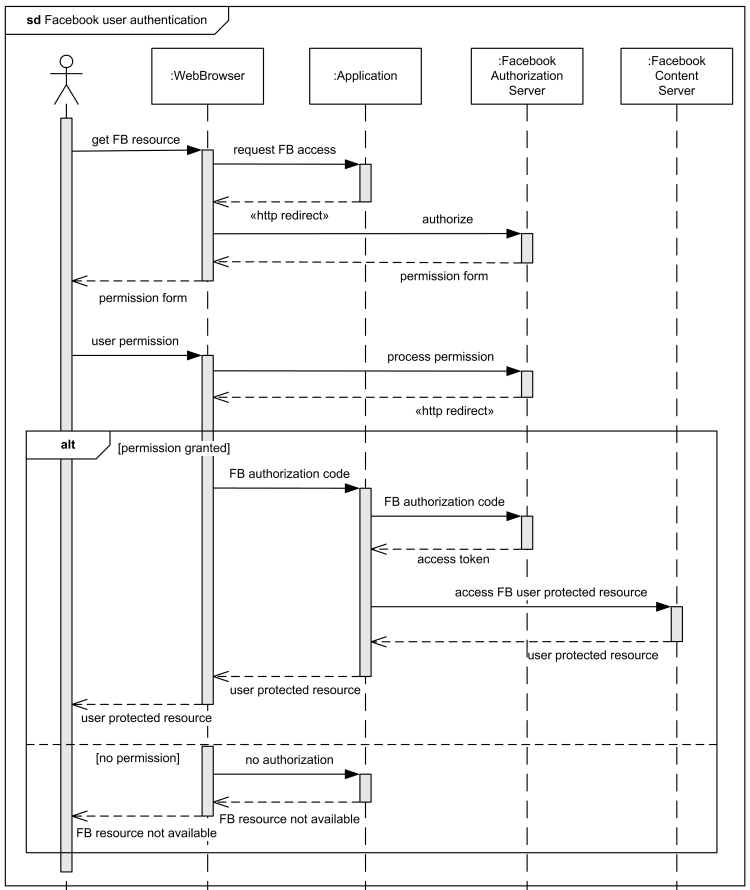
\includegraphics[width=4in]{fb-uml.png}

Explain what happens if the user did not authorize web application.

Sketch: Facebook issues redirect request to the URI specified before, and 
adds the error\_reason parameter to notify the web application that authorization request was denied.

\vfill

\newpage
\question UNIX

\begin{parts}
\part[3] Explain the difference between a built-in shell command, and a regular program
that is executed by the shell. Give examples of each.

Sketch: A built-in is executed by code within the shell, i.e., within the same process.
E.g., printenv, pwd, cd, echo, etc.
When the shell runs a regular program it uses a system command  (fork or vfork) to
create a new process that runs that program. E.g., grep, java, any C program you write, etc.

\vfill
\vfill
\vfill

\part[6]  Explain what each of these commands does:
\begin{itemize}
\item ps (Sketch: lists information about processes running on the system)
\vfill
\item grep (Sketch: finds text within a file)
\vfill
\item wc (Sketch: reports the size of a file, including number of lines and words)
\vfill
\item sort (Sketch: sorts the input, typically stdin. Basic unit of sorting is a line.)
\vfill
\item find (Sketch: search for files in a file system matching optional constraints on size, 
prefix, suffix, permissions, etc.)
\vfill
\item ls (Sketch: list files in a directory)
\vfill
\end{itemize}
\vfill
\end{parts}

\newpage

\question[10] UNIX

Write a shell script for efficiently finding files in a directory and all its nested subdirectories
which are duplicated. Your program
should take a single argument which is a string $s$ of file sufffixes
separated by commas. Any file whose suffix is in the set denoted by $s$ should
be ignored. E.g., if $s$ is ``.png,.jpg,.tar'' then if two files a.png and b.png 
are identical, you should not report them.

The md5 and diff programs, which are a part of any UNIX install may be useful. md5 takes
a file as an argument and returns hash code:
\begin{verbatim}
% md5 midterm-sp-2014.tex
MD5 (midterm-sp-2013.tex) = 14b0e0932bba011b59217782402be268
\end{verbatim}
It is extremely fast and accurate (i.e., if files are different their md5 checksums are very very likely
to be different).

diff can be used to check if binary files are different:
\begin{verbatim}
% diff a.tar b.tar
Binary files a.tar and b.tar differ
% echo $?
2
\end{verbatim}

Syntactically correct shell code is not essential, but you should go beyond English, flowcharts, 
and/or pseudo-code. You can choose whatever format you want to present the output.

Update: here's Marty's (almost) one-liner:
\begin{verbatim}
#!/bin/bash
filter=`echo $1 | sed 's/,/\|/g'`
find -type f -exec md5sum '{}' ';' | sort \
  | uniq -D -w 33 | cut -c 35- | egrep -v $filter
\end{verbatim}

\newpage Overflow page for UNIX shell script question

Sketch: very similar to the UNIX quiz exercise in lab. Get the list of files, use md5 to generate
their checksums, pipe this list through sort, which will put all files which have the same 
checksum together. 

In reality, this is enough, two files which have the same checksum will be the same (probability of
their being different is 1 in $2^{128}$).

If you are paranoid, you can use the return code from diff to confirm if
files with the same checksum are infact equal.the return code from diff to confirm if
files with the same checksum are infact equal.

\newpage
\question[6] Design Patterns

You come across Java code for a class that represents maps. 
The constructor takes a large number of strings as arguments. 
It is very common for most of the strings to be passed in as null.
Explain what problems might arise with such a constructor and 
how the Builder pattern  might be used to solve these problems.

Sketch: problem is it's hard to remember what each argument is supposed to be,
and to swap arguments (since their types are the same).

Solution is to use a Builder pattern. 
Make the constructor private, have an inner class with methods that make the
construction process easier, e.g., getter and setter type
methods.  A build step returns the object. This last step can check for invariants
that must hold of the object.

\vfill
\question[6] Design Patterns

Explain the Singleton Pattern. Specifically, describe
where it is used, and give Java code illustrating a basic implementation
of a singleton class.
\vfill

Sketch: Singleton ensures a class only has one instance, and provides a global
point of access to it. Singleton pattern is used for some classes to have
exactly one instance. For example, there should be only one file system and one
window manager. 

Eager initialization
\begin{verbatim}
public class Singleton {
    private static final Singleton instance = new Singleton();
    private Singleton() {}
    public static Singleton getInstance() {
        return instance;
    }
}
\end{verbatim}

Lazy initialization
\begin{verbatim}
public class Singleton {
    private static volatile Singleton instance = null;
    private Singleton() {}
    public static Singleton getInstance() {
        if (instance ==  null) {
            synchronized(Singleton.class) {
                if (instance == null) {
                    instance = new Singleton();
                }
            }
        }
        return instance;
    }
}
\end{verbatim}

\newpage
\vfill
\question[6] Design Patterns

Explain the concept of Abstract Factory using the Lab Exercise on Pizzas as an example.


Sketch: Abstract factory provides an interface for creating families of related 
or dependent objects without specifying their concrete classes.

In the Lab Exercise, NYPizzaIngredientFactory and ChicagoPizzaIngredientFactory
are two concrete subclass of IngredientFactory. Each subclass implements the
operations to create the appropriate ingredients. For example, the
createCheese operation on the NYPizzaIngredientFactory instantiates and 
returns a MozzarellaCheese, while the corresponding operation on the
ChicagoPizzaIngredientFactory returns a ReggianoCheese. PizzaStore creates
ingredients solely through the IngredientFactory interface and have no 
knowledge of the classes that implement ingredients for a particular look and 
feel. In other words, PizzaStore only have to commit to an interface defined by 
an abstract class, not a particular concrete class.
\end{questions}

\end{document}
